\chapter{Introducción específica} % Main chapter title

\label{Chapter2}

%----------------------------------------------------------------------------------------
%	SECTION 1
%----------------------------------------------------------------------------------------
En este capítulo se profundiza en conceptos de negocio que es importante comprender para el desarrollo del trabajo y se detallan los requerimientos. Adicionalmente, se brinda más información sobre los modelos de inteligencia artificial y otras herramientas empleadas en la solución.

\section{Variables y reglas de negocio}
\label{sec:Negocio}

El Banco de Crédito del Perú es el banco más grande de su país con más de 11 millones de clientes y más de 17 mil empleados. Cuenta con diversas áreas de negocio repartidas según canales de atención, segmentos de clientes o productos. Por ejemplo, existen equipos de trabajo para canales alternativos como cajeros, para segmentos de clientes afluentes y para productos hipotecarios o de medios de pago, entre muchos otros. Cada uno de estos tiene analistas de negocio que se encargan de gestionar campañas comerciales o proyectos, y muchos de ellos exigen comunicaciones a los clientes. El email es uno de los principales canales de comunicación que se eligen ya que no implica uso del presupuesto de área y es relativamente fácil de gestionar. Sin embargo, la mayoría de los pedidos de correos son derivados a un solo equipo de diseño, quien muchas veces debe priorizar y postergar algunos pedidos por falta de capacidad.

El equipo de diseño desarrolla los emails con base en \textit{briefs}. En el caso de campañas grandes que exigen varios canales de comunicación y una estrategia más compleja, se tienen \textit{briefs} más extensos. Pero en general, para emails tácticos, se utiliza un \textit{mini-brief} que incluye estas preguntas:

\begin{enumerate}
    \item Objetivo de la campaña.
    \item ¿Quién es nuestro público objetivo?
    \item ¿Qué queremos decirles?
    \item ¿A qué segmentos va dirigido? Si incluye ENALTA, confirmar la firma de quién irá en el mail.
    \item Tipo de piezas y mandatorios.
\end{enumerate}

Las tres primeras preguntas ayudan a dar contexto sobre qué se quiere lograr con la comunicación, cómo adaptarla según el público al que va dirigida y detalla el contenido del email. La cuarta pregunta pide especificar el segmento del cliente.

Dentro del banco, existen diferentes segmentos de clientes personas naturales que se definen principalmente sobre la base de los ingresos y patrimonio de estos. De menos a más ingresos, estos son los segmentos: 
\begin{itemize}
    \item Consumo.
    \item Banca Exclusiva (BEX).
    \item Enalta.
    \item Privada.
\end{itemize}

Cada segmento tiene colores y diseños de emails ligeramente diferentes. En específico, Enalta y Privada tienen incluso sus propios logos. Adicionalmente, los cierres de los emails cambian. En Consumo, el cierre es más general y se derivan las consultas a canales de atención masivos. Para el resto de los segmentos, los cierres derivan las consultas a los funcionarios asignados a cada cliente en específico, por lo que en el código HTML se incluyen campos personalizables para estos casos. Para el alcance del presente trabajo se consideraron solo los segmentos Consumo y BEX, ya que abarcan la mayoría de clientes. 

En las figuras~\ref{fig:EjConsumo} y~\ref{fig:EjBEX} se pueden visualizar ejemplos de las variantes de emails de una misma campaña para estos dos segmentos. Adicionalmente, se puede observar un análisis inicial de las partes que componen un correo, lo que es crucial para el desarrollo de la solución. Como se puede notar, la cabecera y el cierre son los que más variaciones tienen entre Consumo y BEX. Además, a veces se presentan cambios en el color del texto para resaltar frases importantes.

Otra sección del correo que es relevante considerar son los Términos y Condiciones (T\&C) y los legales. Los T\&C son opcionales y los analistas de negocio los tienen que compartir textualmente en el \textit{brief}. Estos se incluyen sin ninguna modificación en el email, ya que han sido revisados previamente por el área de legal. Adicionalmente, existe un texto genérico que se incluye en todos los emails del banco (los dos últimos párrafos). Este legal genérico no es necesario mencionarlo en el \textit{brief} ya que el equipo de diseño siempre lo incluye en los correos como parte de los lineamientos que tiene. 

Por último, para comunicaciones de productos que tienen asociadas tasas, es necesario incluir tasas referenciales en el legal. La tasa especificada puede ser tasa de costo efectiva anual (TCEA) para productos activos (aquellos que involucran que el banco preste dinero al cliente), o tasa de rendimiento efectiva anual (TREA) para productos pasivos (aquellos en los que el cliente deja su dinero en custodia del banco). Tanto la tasa como su descripción también deben ser brindadas por el analista de negocios en el \textit{brief}.

\cleardoublepage
\begin{figure}[!htpb]
     \centering
     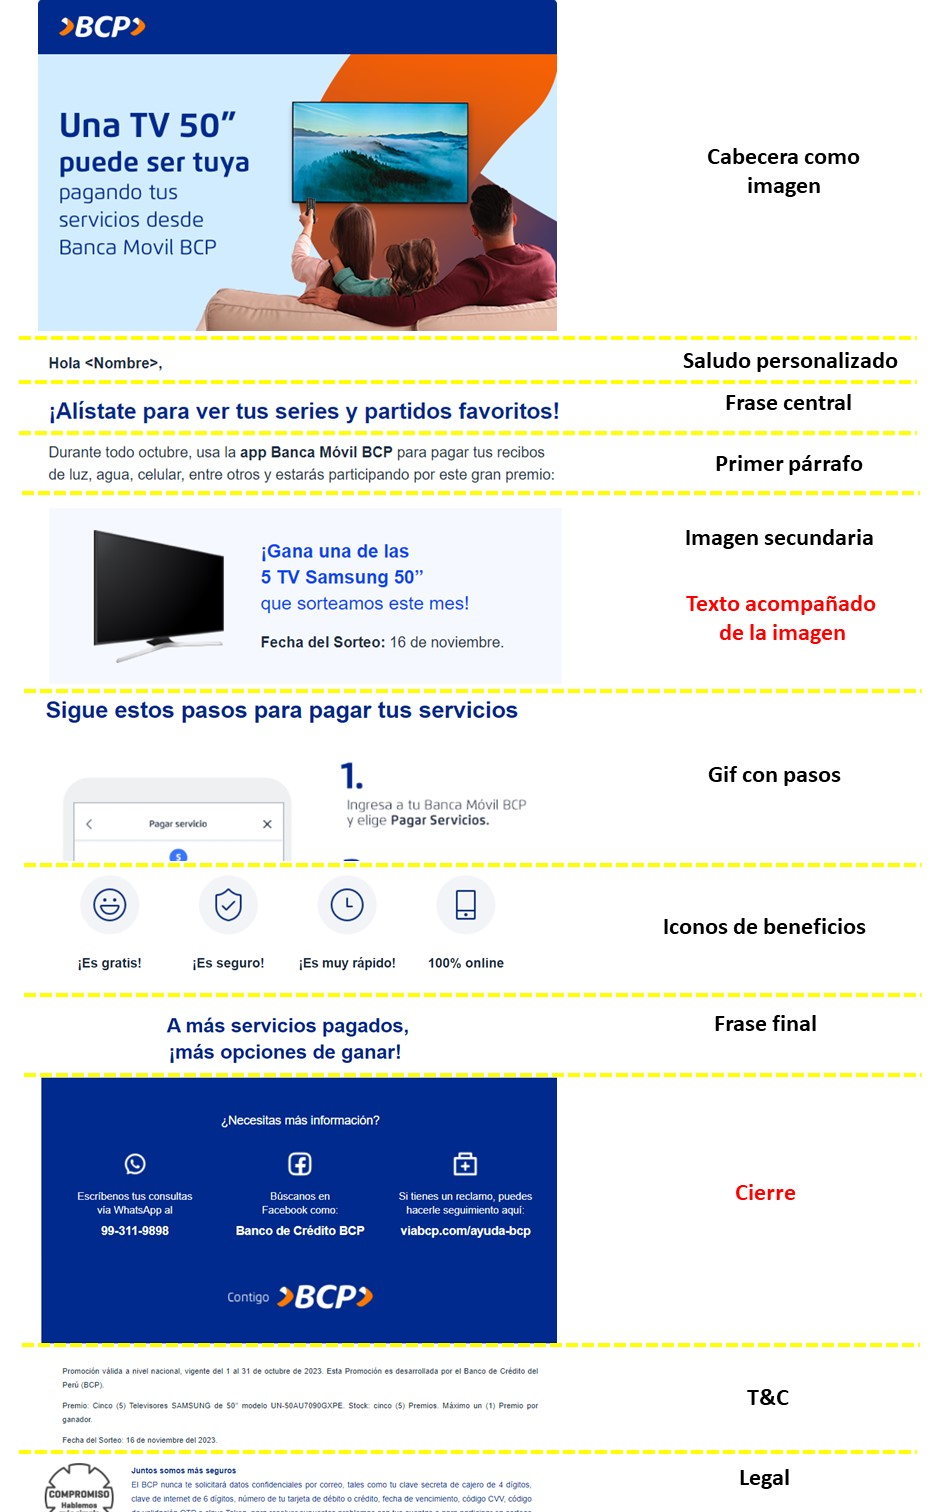
\includegraphics[width=1\textwidth]{./Figures/ejemplo_Consumo}
    \caption{Ejemplo de email para Consumo.}
    \label{fig:EjConsumo}
\end{figure}

\begin{figure}[!htpb]
     \centering
     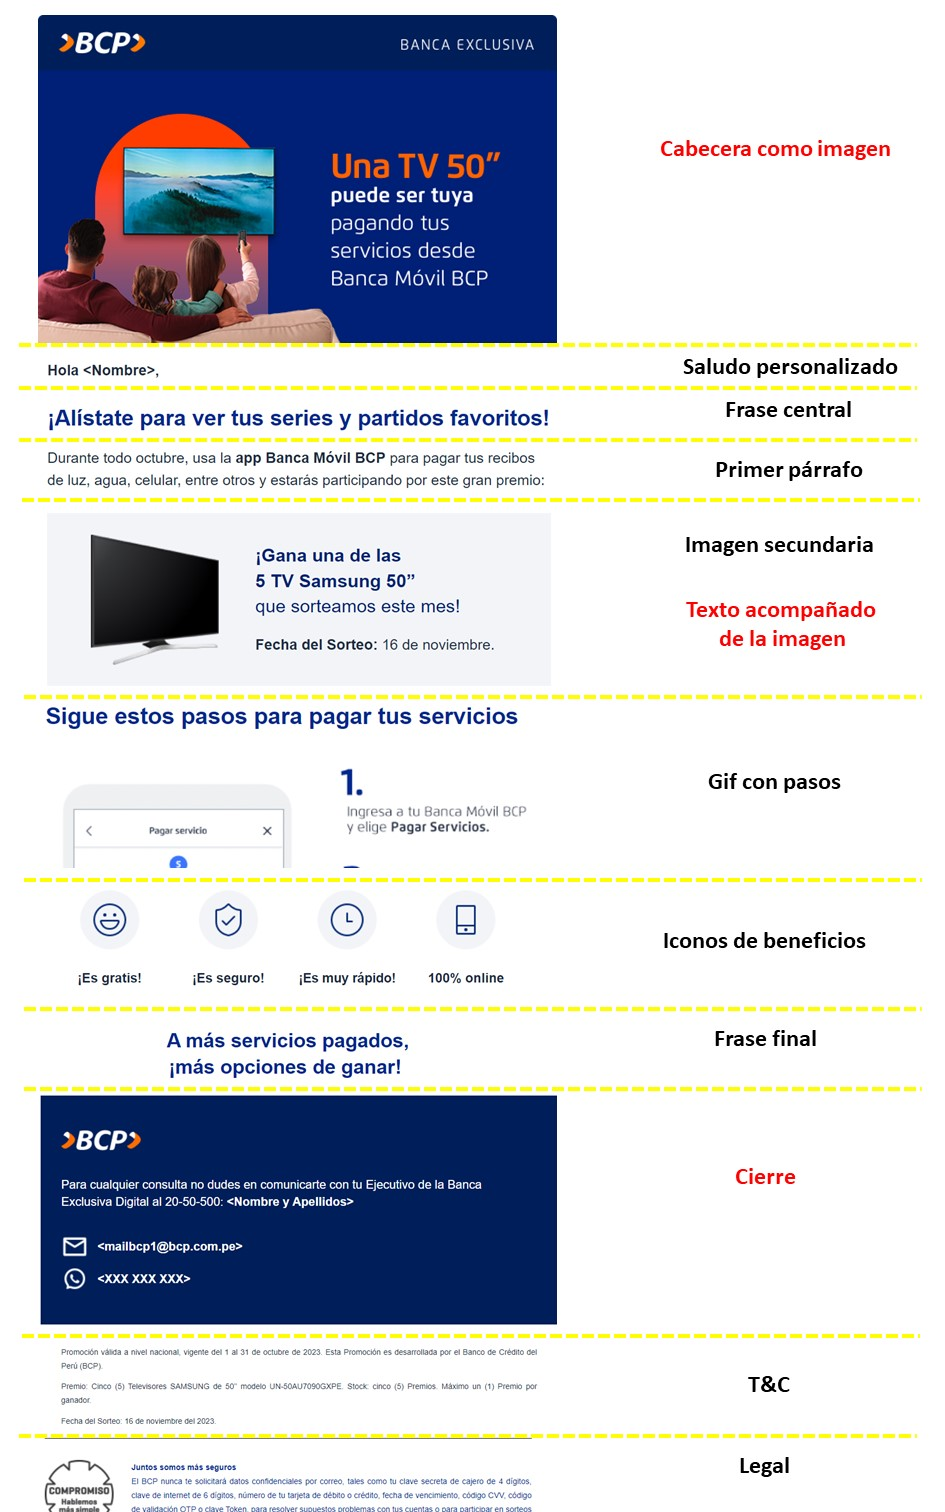
\includegraphics[width=1\textwidth]{./Figures/ejemplo_BEX}
     \caption{Ejemplo de email para BEX.}
     \label{fig:EjBEX}
\end{figure}


\section{Requerimientos}

Los requerimientos que se han considerado al momento de desarrollar el presente trabajo fueron los siguientes:

\begin{enumerate}
	\item Requerimientos funcionales:
		\begin{enumerate}
			\item El sistema debe generar un boceto de email según la información brindada en un \textit{brief} que incluye: 1) Objetivo de la campaña 2) Público objetivo 3) Mensaje que se desea comunicar.
			\item El formato final del proceso es un archivo index.html con una carpeta ``img"  que contenga las imágenes necesarias para el email. Este formato es compatible con Adobe Campaign.
			\item Se debe generar un \textit{output} intermedio que permita al usuario revisar el contenido del email antes de su versión final.
			\item El email generado debe cumplir con los lineamientos de diseño de la empresa, considerando que el formato varía según los segmentos de clientes.
		\end{enumerate}
	\item Requerimientos de confidencialidad y seguridad:
		\begin{enumerate}
			\item La información de la empresa brindada para entrenar el modelo no debe ser compartida con terceras empresas.
			\item La información que se comparte al modelo mediante los \textit{briefs} no debe contener datos de alta criticidad de clientes o personas (número de documento, nombres, datos de contacto, entre otros).
		\end{enumerate}
	\item Requerimientos de la interfaz:
		\begin{enumerate}
			\item El modelo debe poder ser utilizado por usuarios no técnicos pertenecientes a equipos de diseño y marketing.
		\end{enumerate}
\end{enumerate}

\section{Modelos de generación de texto utilizados}

En esta y en la siguiente sección (\ref{sec:modelosimagenes}) se describen los modelos y herramientas que se utilizan en este trabajo y que permiten alcanzar los requerimientos mencionados. Uno de los retos más importantes fue poder generar tanto texto como código HTML. Como se mencionó en la sección \ref{sec:estadodelarte}, los avances en grandes modelos de lenguaje (LLMs, por su sigla en inglés) son los que hicieron posible esta solución. A continuación, se profundiza acerca de los LLMs y cuáles están disponibles. Además, se brinda información sobre varias herramientas que se derivan de estos modelos, como las APIs de LLMs, agentes AI y marcos de trabajo como LangChain \cite{langchain}.

\subsection{Grandes modelos de lenguaje}

Los grandes modelos de lenguaje son modelos de aprendizaje profundo entrenados con grandes cantidades de texto para predecir la probabilidad de secuencias de palabras. Se les llama "grandes" por los miles de millones de parámetros que manejan, lo cual les permite aprender patrones y estructuras complejas del lenguaje natural \cite{Vaswani2017}. Utilizan \textit{tokens}, que son unidades básicas de texto (como subpalabras o símbolos), para procesar y generar lenguaje \cite{Vaswani2017}. Actualmente, los LLMs se emplean para una variedad de tareas como la generación de texto, la traducción automática, la respuesta a preguntas y la síntesis de texto.

Entre los LLMs más destacados disponibles actualmente se encuentran GPT-4 \cite{OpenAIGPT4}, Claude \cite{AnthropicClaude}, GPT-3.5 \cite{OpenAIGPT35}, Vicuna \cite{LMSYSVicuna}, y LLaMA \cite{MetaLLaMA}, entre otros. Algunos de estos modelos son de código abierto, como Vicuna y LLaMA, mientras que otros son privados, como GPT-4. Un estudio reciente \cite{zheng2023judging} comparó estos modelos utilizando tanto jueces humanos como los propios LLMs para determinar cuál es mejor en diversas tareas. En este estudio, GPT-4 fue uno de los modelos ganadores, mostrando un rendimiento superior en varias métricas. En la figura~\ref{fig:comparacionLLMS} se observa la tasa de victorias promedio de nueve modelos bajo diferentes jueces.

\begin{figure}[h]
  \centering
  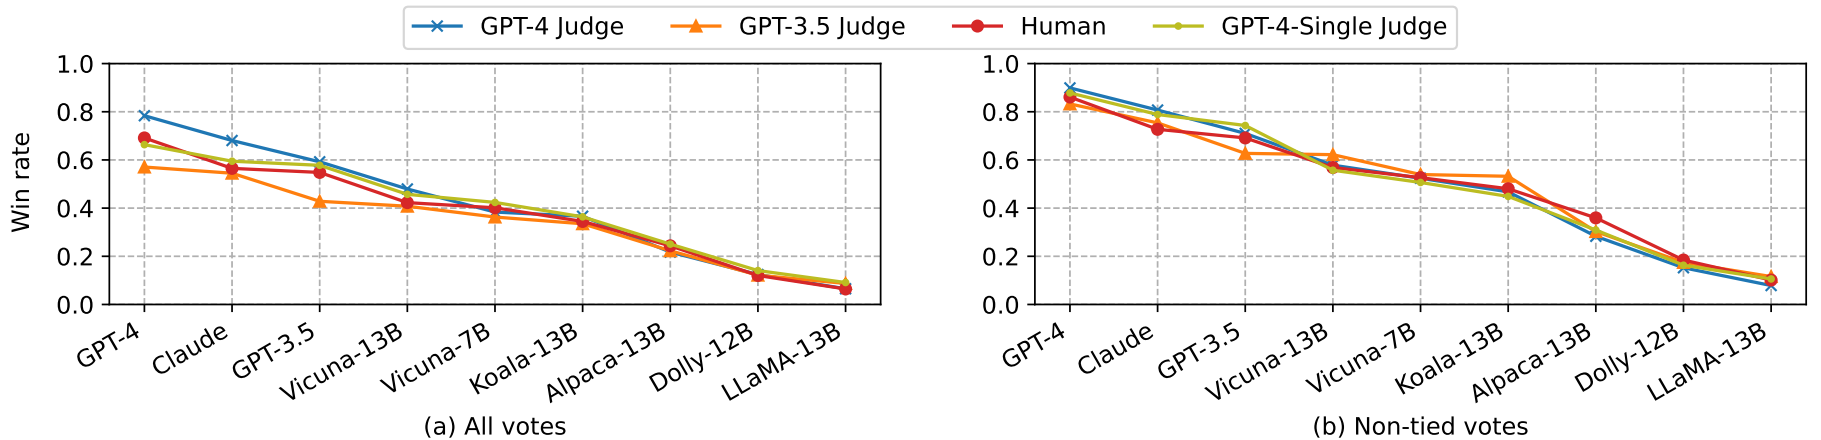
\includegraphics[width=\linewidth]{./Figures/comparacion_LLMs.png}
  \caption{Tasa promedio de victorias de nueve modelos bajo diferentes jueces\protect\footnotemark.}
  \label{fig:comparacionLLMS}
\end{figure}

\footnotetext{Imagen tomada del paper \textit{Judging LLM-as-a-Judge
with MT-Bench and Chatbot Arena} \cite{zheng2023judging}}

\subsection{API de OpenAI}

Varias LLMs privadas están disponibles para su uso mediante APIs. Por ejemplo, OpenAI ofrece una API que permite acceder a modelos como GPT-4o, GPT-4 y GPT-3, entre otros. Mediante esta se pueden enviar consultas a los modelos y recibir el texto generado como respuesta. Además, existen funcionalidades como el modo JSON que permiten estructurar las respuestas de tal forma que sirvan de \textit{input} para otros procesos dentro del aplicativo que se esté construyendo \cite{openai}.

El cobro por el uso de la API se realiza en base a la cantidad de \textit{tokens} de entrada y salida procesados. El usuario genera un API \textit{key} que se brinda al momento de enviar cualquier solicitud a la API, de tal forma que se pueda medir el uso asociado a esa llave. Adicionalmente, el costo de los \textit{tokens} varía en función del modelo utilizado. En este trabajo, se utiliza GPT-4o mini, ya que es un modelo más reciente que GPT-4 y tiene costos por \textit{token} más económicos \cite{openai}.

\subsection{LangChain y agentes de IA}
\label{sec:LagchainAgentes}

LangChain es un marco de trabajo diseñado para facilitar el desarrollo de aplicaciones que utilizan LLMs. Su utilidad radica en que proporciona herramientas y abstracciones para conectar modelos de lenguaje de diferentes proveedores (como OpenAI) con otras fuentes de datos y sistemas. Además, LangChain permite crear procesos utilizando cadenas. Estas funcionan conectando diferentes componentes que procesan y transforman datos en pasos secuenciales. Esto permite la creación de flujos de trabajo complejos y personalizados \cite{langchain}.

Mediante LangChain también se pueden crear agentes de inteligencia artificial. Un agente de IA es un sistema que puede percibir su entorno y tomar acciones para alcanzar objetivos específicos. Estas acciones las puede realizar gracias a que los agentes tienen a su disposición herramientas (\textit{tools}). Estas son muy poderosas, ya que con ellas la inteligencia artificial ya no se limita a generar texto, sino que puede ejecutar funciones personalizadas. Estas pueden ser creadas por el usuario de la API en lenguajes de programación como Python. Gracias a ellas, los agentes pueden hacer búsquedas por Internet, utilizar calculadoras, hacer consultas a otras APIs, entre otras acciones \cite{langchain}.

\section{Modelos de generación de imágenes utilizados}
\label{sec:modelosimagenes}

Un segundo reto que se tuvo en el desarrollo de este trabajo fue el de generar imágenes que puedan ser incluidas en las cabeceras de los emails. A continuación, se describen los modelos y herramientas que sirven para este propósito.

\subsection{Stable Image Core y Stable Image Ultra}


Stability AI es una empresa de inteligencia artificial que se especializa en el desarrollo de tecnologías para la generación de contenido digital. Uno de sus servicios de generación de imágenes es Stable Image Core \cite{stabilityai2023stable}. Este servicio utiliza por detrás el modelo Stable Diffusion que ha sido creado empleando una combinación de redes U-Net, autoencoders variacionales y procesos de difusión \cite{rombach2022high}. Además, ha sido entrenado en un vasto conjunto de datos de imágenes y textos. Esto le permite comprender y traducir descripciones complejas en imágenes visualmente atractivas, con detalles finos y coherencia contextual \cite{stabilityai2023stable}.

Este servicio ofrece una API que permite a los usuarios enviar un \textit{prompt} (una descripción textual) para generar una imagen correspondiente. Esta API también admite opciones avanzadas como el \textit{negative prompt}, que ayuda a refinar los resultados excluyendo ciertos elementos no deseados de la imagen generada. Además, los usuarios pueden especificar el aspecto de la imagen y el formato de salida, lo que proporciona flexibilidad y control sobre el resultado final \cite{stabilityai2023api}.

Otra alternativa brindada por Stability AI es el API de Stable Image Ultra que es su servicio más avanzado de generación de texto a imagen. Es similar a Stable Image Core pero con varias mejoras. Entre ellas, tiene una comprensión de \textit{prompts} superior, sobresale en tipografía, composiciones complejas, iluminación dinámica, tonos vibrantes, y en la cohesión y estructura general \cite{stabilityai2023ultra}. Debido a que es mejor en varios aspectos, el costo por imagen también es más alto, por lo que en este trabajo se probaron ambas opciones de tal forma que se pueda comparar cuál es mejor para el objetivo planteado.

\subsection{Herramientas de edición de imágenes}

Stability AI también proporciona herramientas para editar las imágenes generadas. A continuación se detallan varias de ellas:
\begin{itemize}
    \item \textit{ESRGAN} (\textit{Enhanced Super-Resolution Generative Adversarial Networks}): es una herramienta de ampliación (escalado), es decir, que aumenta el tamaño de la imagen sin perder calidad \cite{stabilityai2023upscale}.

    \item \textit{Inpainting}: permite rellenar áreas faltantes o dañadas de una imagen basándose en el contexto circundante \cite{stabilityai2023tools}.
    
    \item \textit{Outpainting}: extiende una imagen más allá de sus bordes originales, añadiendo contenido nuevo que mantiene la coherencia con la imagen existente \cite{stabilityai2023tools}.
    
    \item Búsqueda y reemplazo: permite identificar y sustituir elementos específicos dentro de una imagen \cite{stabilityai2023tools}. 
    
    \item Eliminación de fondo: facilita la creación de imágenes con fondos transparentes o nuevos, mejorando la versatilidad y aplicación de las imágenes generadas en diversos contextos \cite{stabilityai2023tools}.
\end{itemize}
